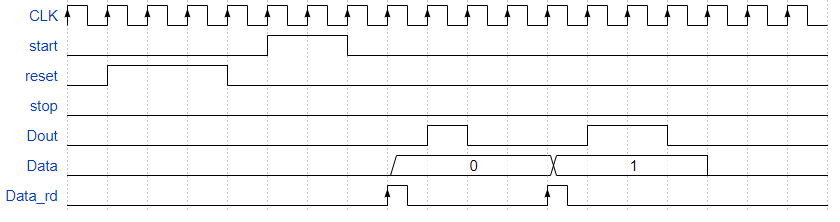
\includegraphics[scale=0.6]{general.PNG}

\begin{itemize}
\item CLK: 100 MHz-es órajel
\item start: jel a folyamat elindításához
\item reset: jel a folyamat resetálásához
\item stop: jel a kiírás megállításához. Csak két 24 bit-es blokk kiírása közben tudja megállítani a kiírást
\item Dout: Egyszálú adatsín a LED-ekre.
\item Data: Kiírandó adat, Data\_rd felmenő órajelére olvassa be az adatot.
\item Data\_rd: Aktiváló bit az adat beolvasására
\end{itemize}

\textbf{2019.11.11}

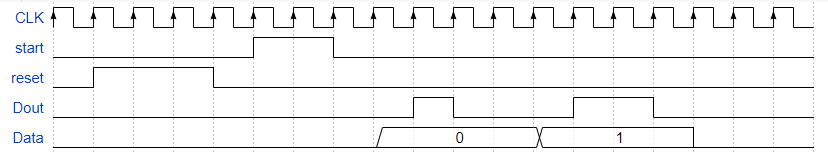
\includegraphics[scale=0.6]{general2.PNG}

\begin{itemize}
\item CLK: 100 MHz-es órajel
\item start: jel a folyamat elindításához
\item reset: jel a folyamat resetálásához
\item Dout: Egyszálú adatsín a LED-ekre.
\item Data: Kiírandó adat
\end{itemize}